\documentclass[11pt, a4paper]{report}
\usepackage[hidelinks]{hyperref}
\usepackage{graphicx}
\usepackage{float}
\usepackage{subcaption}
\usepackage{tabularx}
\usepackage{acro}
\usepackage{fancyhdr}
\usepackage{lipsum}
\usepackage{comment}
\usepackage{markdown}
\usepackage{longtable}
\usepackage{hyperref}
\usepackage{geometry}
\usepackage{array}
\usepackage[natbibapa]{apacite}
\bibliographystyle{apacite}
\geometry{left=3cm,right=3cm, bottom=3cm, top=3cm}

% Font
\setlength{\parindent}{0em}
\setlength{\parskip}{1em}

% fancyhdr
\pagestyle{fancy}
\fancyhf{}
\lhead{\leftmark}
\cfoot{\thepage}
\setlength{\headheight}{13.59999pt}

\begin{document}

\begin{titlepage}
    \centering
    
    \vspace{1cm}
    
    {\scshape\Large INSTITUTE OF GEOGRAPHICAL SCIENCES\par}
    \vspace{1cm}
    
    {\scshape\Large B. Sc. Geographical Sciences\par}
    \vspace{1cm}
    
    \vfill
    {\huge\bfseries Bachelor's Thesis\par}
    
    {\large\bfseries Spatial Accessibility to Healthcare Facilities in the Tri-Border of the Alto Paraná Atlantic Forest}
    \vfill
    
    {Submitted by\par}
    {\Large Joaquin Gottlebe \par}
    {5429130}
    \vspace{1cm}
    
    {First supervision by \par}
    {\Large Jun.-Prof. Dr. María Piquer-Rodríguez\par}
    {Second supervision by \par}
    {\Large Dr. Lia Montti\par}
    {Co-advised by \par}
    {\Large M.Sc. Ahuvit Trumper \par}
    \vspace{1cm}
    
    {Berlin, Germany\par}
    {\today\par}
    
\end{titlepage}

\pagenumbering{Roman}

\chapter*{Declaration of Academic Integrity}

I hereby declare to the Freie Universität Berlin that I have completed the following Bachelor's Thesis independently and without the use of sources and aids other than those cited.

I declare that the present work is free of plagiarism. Any statements that have been taken from other writings, whether directly or indirectly, have been clearly marked as such. 

No entire section or full paragraph of this thesis was written with the help of an AI. If an AI was used, was only to improve my own writing.

Further, I declare that this work has not been submitted to any other university as part of an examination attempt, either in identical or similar form, nor has it been published elsewhere.

\vfill

{
\centering

Berlin, Germany 

\today

\vspace{4em}

\underline{\hspace{6cm}}

Joaquin Gottlebe

5429130

}

\vfill

\chapter*{Acknowledgements}

Firstly, I want to express my heartfelt gratitude to my first supervisor, Jun.-Prof. Dr. María Piquer-Rodríguez, for your support, insightful feedback, and patience throughout this journey. Your expertise has been invaluable. I also extend my thanks to my second supervisor, Dr. Lia Montti, for your support, extensive knowledge of the study area, and kind words. My appreciation goes to M.Sc. Ahuvit Trumper for your support from day one and for laying the groundwork for this research. I am grateful to the entire "Modelling Human-Environmental Interactions" working group at the Freie Universität Berlin for being the best colleagues I could ask for. I also want to thank Theresa for her emotional support, as well as my family, friends and my cat Kafka for always being there for me. I owe my deepest gratitude to my partner, Rebecca, who is my  beacon of light. And last but not least, as Snoop Dogg famously said, I wanna thank me.

\tableofcontents
\newpage
\listoffigures
\newpage
\listoftables
\newpage
%\chapter*{Acronyms}
%\printacronyms[heading=none, include-classes=abbrev]
%\chapter*{Symbols}
%\printacronyms[heading=none, include-classes=symbols]


\chapter*{Abstract}

This thesis analyses the spatial accessibility of healthcare facilities in the tri-border area of the Alto Paraná Atlantic Forest, which includes municipalities in Paraguay, Brazil and Argentina. The study aims to provide a comprehensive analysis of the differences in accessibility between different regions and population groups in this area. \\
%
Using data from OpenStreetMap, official government sources and the Global Human Settlement Layer, the study combines a friction surface and a cost distance algorithm to model the cost of movement through space and calculate travel time to healthcare facilities as an indicator for accessibility.\\
%
The analyses revealed notable disparities in healthcare accessibility between the three countries with Brazil and Argentina having the highest accessibility, followed by Paraguay with the lowest accessibility. A strong correlation between population density and accessibility revealed that urban regions exhibit the highest accessibility, while rural and peripheral areas, particularly in Paraguay face much lower accessibility. It was also revealed that indigenous communities are negatively influenced greater by these disparities of accessibility.  \\
%

\chapter{Introduction}
\pagenumbering{arabic}
\section{Agenda for Sustainable Development}\label{sec:introagenda}

This thesis is rooted in the third goal of the global Agenda for Sustainable Development by the United Nations, published in 2015 by the \citet{united_nations_transforming_2015}. This Agenda defines 17 sustainable development goals as a comprehensive plan of action, which are a collective commitment to addressing these most pressing global challenges like elevating societal well-being, protecting our planet, creating lasting prosperity and particularly healthcare accessibility. \\
%
Goal 3 specifically calls for equal access to healthcare and education regardless of background, stating: "Ensure healthy lives and promote well-being for all at all ages" \citep{united_nations_transforming_2015}. It emphasises the need for universal healthcare coverage, equitable healthcare services, and improved health outcomes worldwide. This goal is crucial for sustainable development as it improves overall health and increases productivity, which in turn contributes to poverty reduction and economic growth \citet{zhao_economic_2016}. It also promotes equality for marginalised groups \citet{davy_access_2016}. \\
%
Achieving this goal requires a concerted effort from various actors, including governments, international organisations, and non-governmental organisations (NGO's) \citet{sanadgol_engagement_2021}. Key initiatives such as the Universal Health Coverage Partnership of the World Health Organisation (WHO) \citet{uhc-partnership_universal_2021} and the Global Fund to Fight AIDS, Tuberculosis, and Malaria \citet{the_global_fund_global_2024} illustrate the global commitment to improving healthcare accessibility. These initiatives focus on strengthening healthcare systems, improving service delivery, and ensuring that healthcare is accessible to all, especially the most vulnerable  \citet{syed_traveling_2013}. \\
%
One indicator the United Nations uses to measure the progress of the third goal is for example the Universal Health Coverage indicator, which is generated by the WHO \citet{world_health_organization_tracking_2023}. This indicator tracks various aspects of healthcare accessibility, including the availability of essential healthcare services, patient satisfaction, and reduced travel times to healthcare facilities. 

\section{Access to Healthcare}\label{sec:introaccess}
While the Universal Health Coverage indicator provides a broad overview of healthcare accessibility, a deeper understanding of access to healthcare is necessary. Access to healthcare is complex to define and measure, as highlighted by \citet{aday_framework_1974}. They suggest that it is perhaps most meaningful to consider access in terms of whether those who need care receive it. \citet{gulliford_what_2002} similarly define access to healthcare as the ability to obtain appropriate health care resources to maintain or improve health. Both \citet{aday_framework_1974} and \citet{gulliford_what_2002} emphasise the importance of viewing healthcare accessibility as a multidimensional concept. They identified three primary barriers to healthcare access: the personal barrier, which involves patients' recognition of their need for healthcare and their decisions to seek it; the financial barrier, which pertains to the cost of healthcare services and how it influences patients' decisions to obtain care; and the organisational, also called structural barrier, which encompasses all aspects related to the provision and ease of access to healthcare services \citet{gulliford_what_2002}. In detail organisational barriers to healthcare access include structural and systemic barriers such as insufficient resources, inefficient processes, long waiting times, lack of coordination and integration of healthcare services as well as geographical barriers that make access to medical facilities difficult for example the travel time to healthcare facilities \citet{carrillo_defining_2011}.\\
%
According to \citet{wang_assessing_2005}, organisational barriers can arise from spatial variability due to the uneven distribution of healthcare providers and consumers, as well as differences among population groups based on socioeconomic and demographic characteristics, which then causes variability in travel time. \\
%
The consequences of these organisational barriers to healthcare access are examined by \citet{syed_traveling_2013}. They conclude that such barriers can lead to rescheduled or missed appointments, delayed care, and missed or delayed medication use, ultimately resulting in poorer management of chronic illnesses and poorer health outcomes. 

\section{Travel Time}\label{sec:introtraveltime}
A critical factor in understanding the variability in travel time to healthcare services as an organisational barrier is spatial accessibility. It is determined by the barriers or friction of space, which are influenced by the time and physical distance needed to access the services  \citet{aday_framework_1974}. \\
%
To calculate travel time to health care facilities and therefore the accessibility for a region \citet{weiss_global_2018} proposed a method which integrates different datasets and geo-spatial modelling techniques to quantify travel time to urban centres. Nelson \citet{nelson_suite_2019} and \citet{european_commission_joint_research_centre_global_2021} first developed this methodology which \citet{weiss_global_2018} developed further. The authors used data from Open Street Map (OSM) and Google Roads to create a comprehensive road network, supplemented by rail and waterway networks as well as topographic and land cover data. This information was converted into a "friction surface" that represents the speed of movement through each pixel of the earth's surface. A least-cost path algorithm was applied to calculate the travel time from each point to the nearest city. The results were validated by comparing them with travel times from the Google Maps API, where a high level of agreement was found. They further proposed a method for investigating the travel time to healthcare facilities in \citet{weiss_global_2020} which expands on their previous research with adding healthcare facilities to the model.

\section{Study Area}\label{sec:introstudyarea}
As mentioned in the Sustainable Development Goals the most vulnerable countries like developing and middle income countries are facing special challenges \citet{united_nations_transforming_2015}. For a better understanding and to identify barriers of access to healthcare, like travel time, it is especially important to look at these countries. \\
%
Border regions especially are of interest because of there similar physical conditions but sometimes very different governance policies and land use and planing. Because of that the impact of different kind of governance on spatial indicators like travel time and following that also sustainable development can be investigated. They can also serve as a natural experiment for each country that influence each other with the spillover effect described in \citet{piquer-rodriguez_land_2021}, that policies and developments are copied by the other states. The tri-border of the Alto Paraná Atlantic Forest in South America displays such features and is optimal for such research on differences in accessibility to healthcare and was therefore the study area. It lies 55° West and 25,5° and covers area of  $36854 \ km^2$ (\ref{fig:studyregion}). \\
%
The tri-border is also of interest through its high level of inter-connectivity. For example, as \citet{marques_circularidad_2013} \& \citet{cardelli_caso_2021} found, many people regularly move between the border town for healthcare services, shopping, and work. This movement promotes economic growth and regional cooperation among the countries, as highlighted by \citet{arsentyeva_triple_2020}. The historical development of these countries has also significantly shaped the current dynamics of this area, as discussed \citet{lisboa_path_2021}. However, this inter-connectivity is not without its drawbacks. As \citet{martens_ilegalismos_2019} noted, the region also experiences cross-border theft, often driven by poor financial conditions.

\begin{figure}
  \centering
  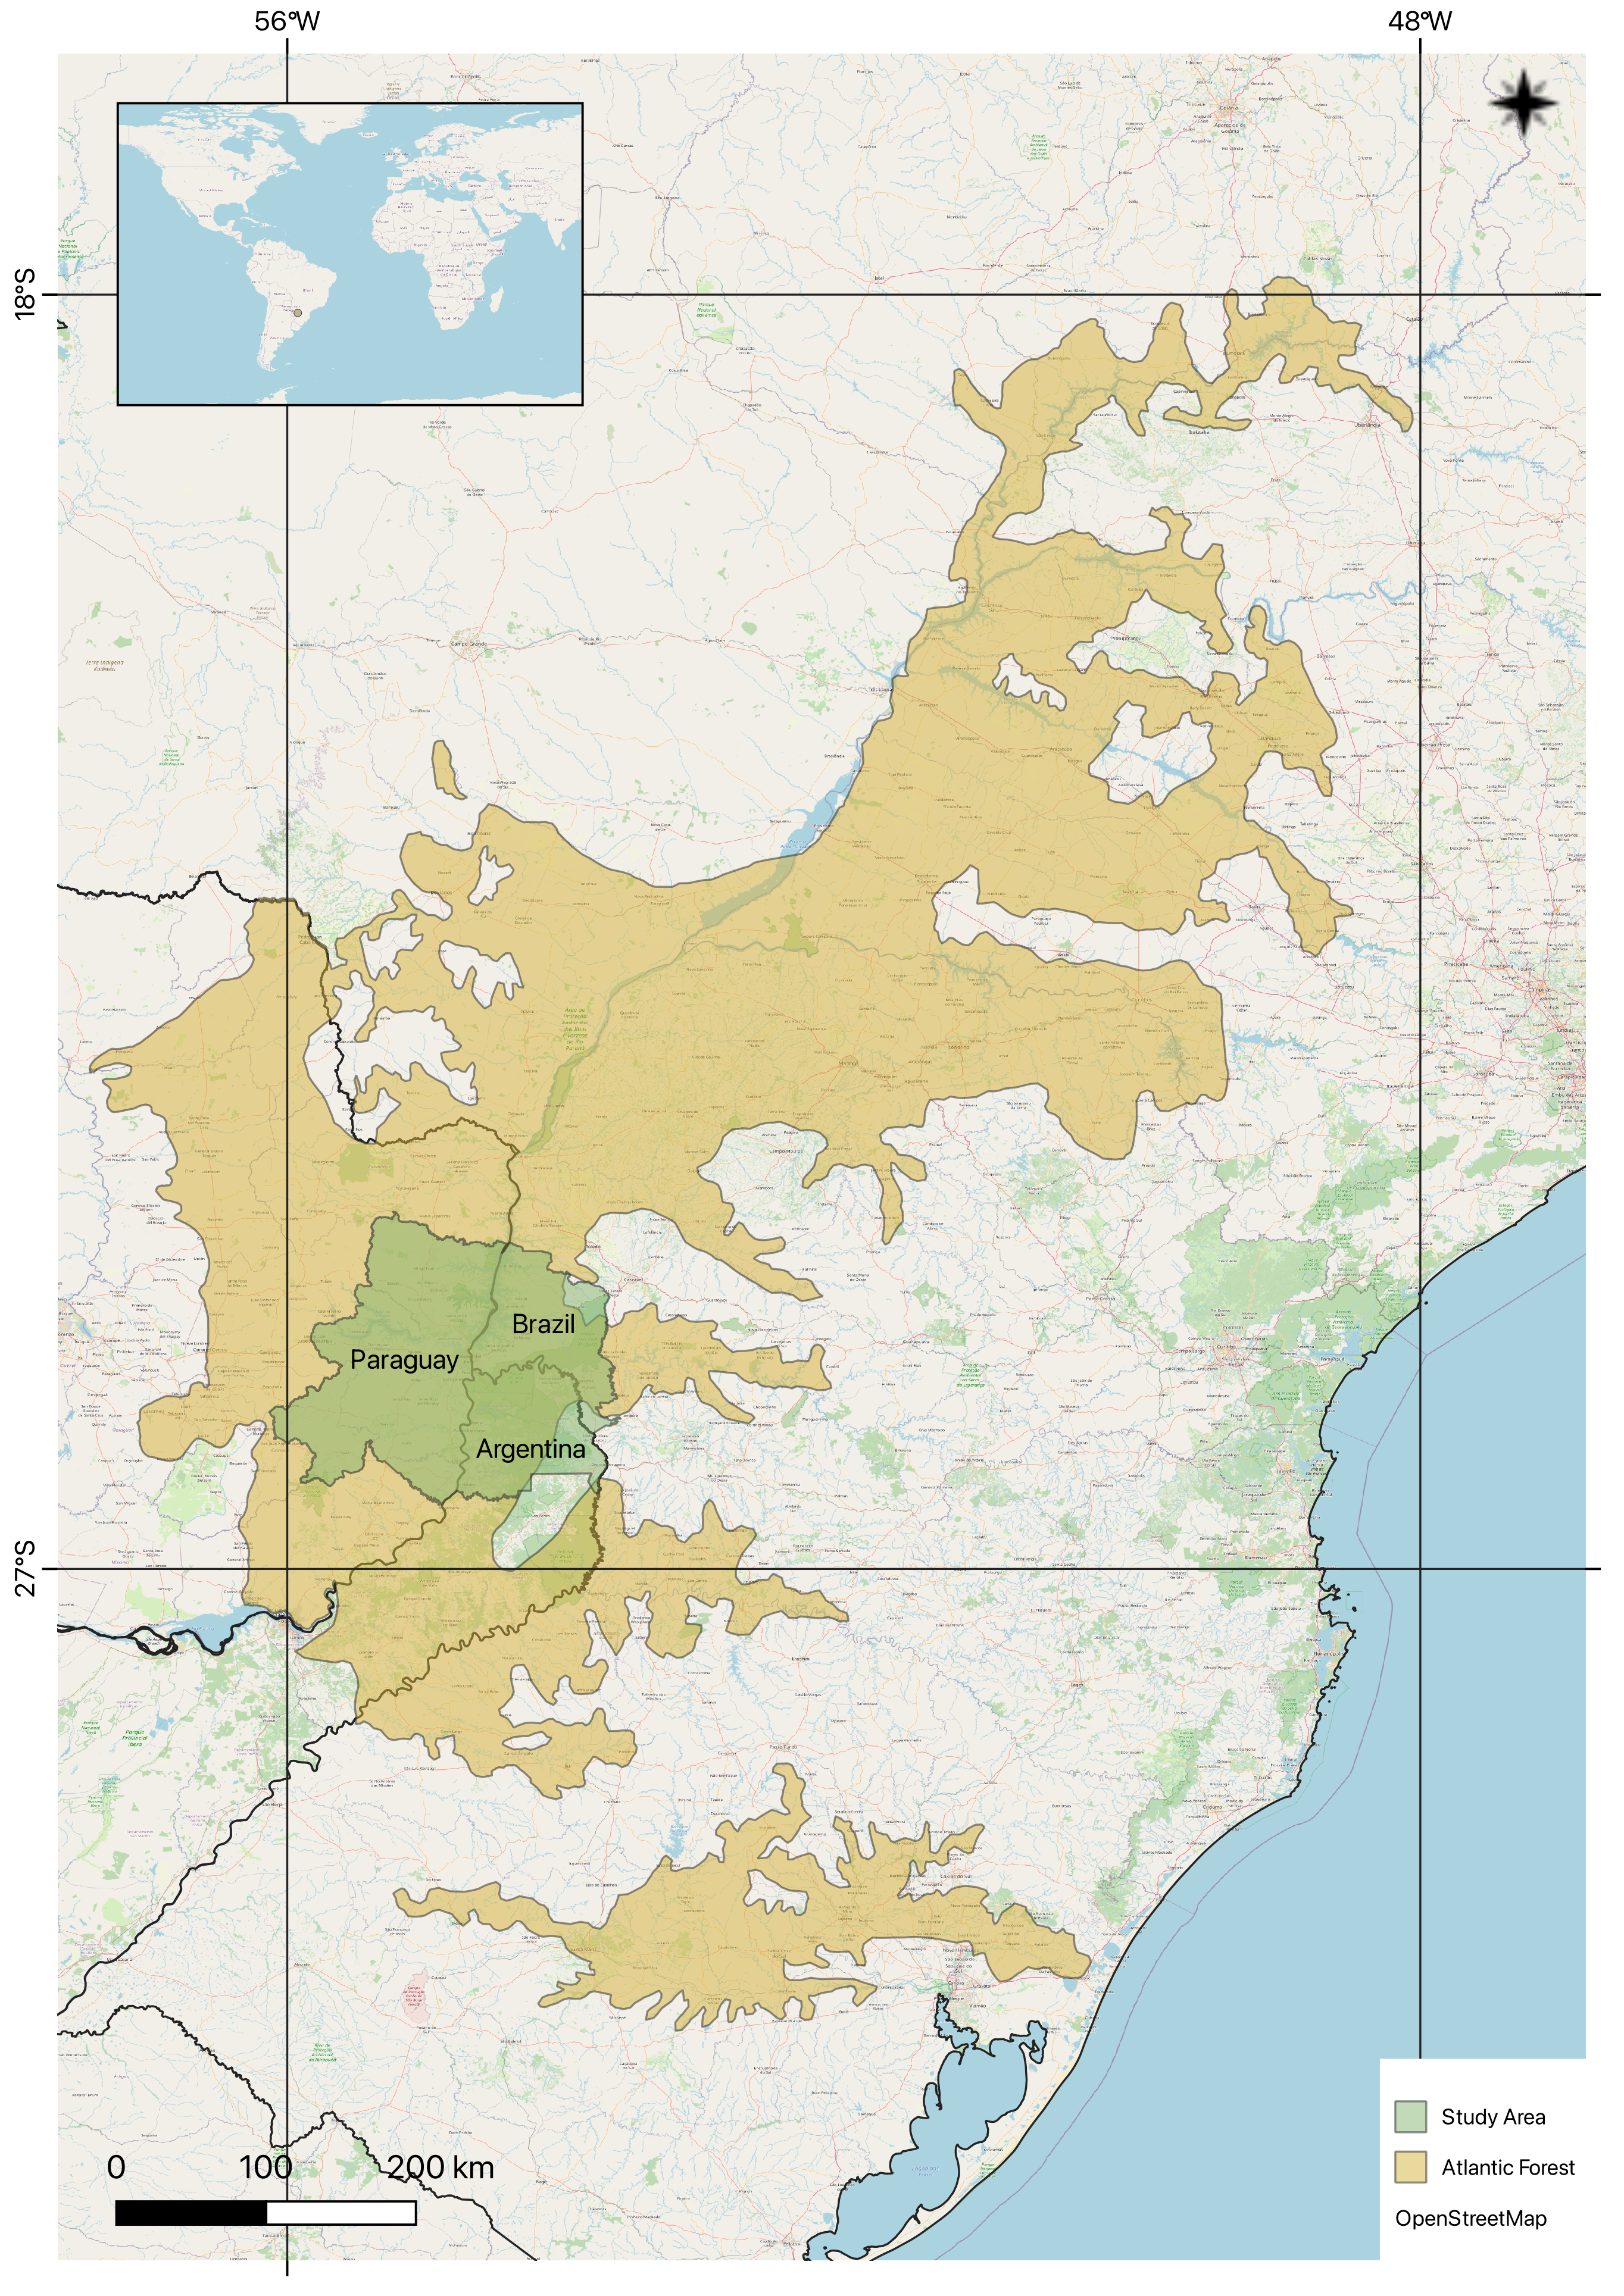
\includegraphics[width=1\linewidth]{figures/Overview.png}
  \caption{Study Region}
  \label{fig:studyregion}
\end{figure}


\subsection{Alto Paraná Atlantic Forest}
The Alto Paraná Atlantic Forest are an important eco-region. This forest extends across the southern part of Brazil, northeastern Argentina and eastern Paraguay. It covers an area of approximately 485,000 km² \citet{schipper_alto_2018}, which is not the study area but surrounds it. The geographical extent of this forest ranges from the coastal forest of the Serra do Mar to the basins of the Paraná River \citet{schipper_alto_2018}. The Alto Paraná Atlantic Forest is of great ecological importance as they have a remarkable biodiversity and endemism \citet{de_lima_erosion_2020}. Despite that, the Alto Paraná Atlantic forest is highly endangered \citet{de_lima_erosion_2020}. Up to 42\% of the original biodiversity and biomass has already been lost in the Atlantic Forest, mainly due to human influence \citet{de_lima_erosion_2020}. These activities have led to a significant fragmentation  of the forest, affecting the habitats of many species and endangering biodiversity \citet{gennerich_land-use_2024}.
The conservation and restoration of the Alto Paraná Atlantic forest is of crucial importance, not only for the protection of biodiversity, but also for the sustainable development of the region. This also extends to the health care of the local population. The loss of forest areas and the associated degradation of ecosystems have a direct impact on the availability and quality of health and well-being through heat stress, as found by \citet{palmer_no_2022}, \citet{hedin_connecting_2022} and \cite{deivanayagam_breaking_2023}. It is therefore important to develop sustainable solutions that ensure both the protection of nature and access to health services. 

\subsection{Argentina}
Argentina's part of the study area consists of three municipalities and covers an area of approximately $7940 \ km^2$. Its border city is Puerto Iguazú. This specific region forms a small part of Argentina's extensive and varied landscape.

The country, is located in the southern half of South America, is the eighth-largest country in the world by land area, covering approximately 2.78 million square kilometres \citet{runfola_geoboundaries_2020}, with over 46 million inhabitants \citet{united_nations_world_2022}. It shares borders with Chile, Bolivia, Paraguay, Brazil, and Uruguay \citet{runfola_geoboundaries_2020}. The country has a diverse geography that includes the Andes mountain range, fertile Pampas plains, and extensive Atlantic coastline.  \\
%
Argentina's population density is approximately 16 people per square kilometre \citet{united_nations_world_2022}.
The country has a high life expectancy of 76 years \citet{world_bank_life_2022}. 
%
Argentina is classified as an upper-middle-income country \citet{world_bank_world_2022}. Its economic instability, characterised by high inflation and fiscal deficits, poses significant challenges to healthcare accessibility, particularly for low-income and vulnerable populations \citet{world_bank_world_2024}. 
Healthcare accessibility in Argentina is also influenced by regional disparities. The healthcare system is divided into public, private, and social security sectors, with the public sector providing free healthcare to all citizens and residents \citet{bello_health_2011}. However, there are significant differences in the quality and availability of healthcare services between urban and rural areas \citet{vacarezza_exploring_2023}, \citet{palacios_need_2020}. The Northwest and Northeast regions, in particular, face challenges in healthcare accessibility due to fewer facilities and healthcare professionals compared to more developed regions like the Pampas \citet{gilardino_access_2016}. Government initiatives such as the Primary Health Care Centres and the Nacer/SUMAR Program aim to improve healthcare access, especially for vulnerable populations \citet{palacios_need_2020}. \\
%
In 2022, Argentina had approximately 955,032 indigenous people, which represents 2.03\% of the total population \citet{berger_indigenous_2024}. The indigenous population in Argentina, faces significant barriers to healthcare access, such as communication and cultural differences, and a lack of essential services like clean water and sanitation\citet{quintana_access_2021}. Initiatives to improve healthcare access for these communities include training community health workers and integrating traditional practices with biomedical care \citet{quintana_access_2021}.

\subsection{Brazil}
Brazil's part of the study area consists of  18 municipalities and covers an area of approximately $8020 \ km^2$. Its border city is Foz do Iguaçu. This area is a small segment of Brazil's vast and varied territory.

It is the largest country in South America, spans an area of 8.5 million square kilometres \citet{runfola_geoboundaries_2020} and is the world's fifth-largest country by both area and population, with over 217 million inhabitants \citet{united_nations_world_2022}. The country is characterised by diverse geographical features, including the Amazon rain forest, Pantanal wetlands, and extensive Atlantic coastline. Brazil's population is heavily concentrated in the southeastern and northeastern regions, with significant urbanisation \citet{agencia_de_noticias_-_ibge_between_2023}. Brazil's population density is approximately 26 people per square kilometre \citet{united_nations_world_2022}. The country has a life expectancy of 73 years \citet{world_bank_life_2022}.  \\
%
Brazil is classified as an upper-middle-income country \citet{world_bank_world_2022}. Its economic disparities, coupled with regional inequalities, significantly impact healthcare accessibility, particularly in under-served and remote areas \citet{hone_effect_2019}.  \\
%
Brazil's healthcare system, known as the Unified Health System (SUS), provides universal healthcare to all residents \citet{oliveira_challenges_2017}. Despite this, there are significant disparities in healthcare access and quality, particularly in rural and remote areas \citet{palmeira_analysis_2022}. The distribution of healthcare facilities and professionals is uneven, with the North and Northeast regions facing greater challenges in accessing healthcare services compared to the more developed Southeast \citet{silva_emergency_2021}. Initiatives such as the Mais Médicos (More Doctors) Program aim to address these disparities by improving the distribution of healthcare professionals across the country \citet{oliveira_challenges_2017}. \\
%
The indigenous population in all of Brazil, consisted  in 2022  of 1,693,535 people, which represents approximately 0.83\% of the total population \citet{berger_indigenous_2024}. The indigenous population includes numerous ethnic groups, faces significant health inequities, including higher infant mortality rates, lower life expectancy, and a high burden of infectious diseases \citet{berger_indigenous_2024} \citet{santos_health_2022} \citet{mendes_o_2018}. The Indigenous Healthcare Subsystem (SASI) and the National Policy for the Care of Indigenous Peoples (PNASPI) aim to provide differentiated healthcare that respects socio-cultural diversity \citet{de_m_pontes_health_2020}. 


\subsection{Paraguay}

Paraguay's part of the study area consists of  29 municipalities and covers an area of approximately $20894 \ km^2$. Its border city is Ciudad del Este. This region represents a portion of Paraguay's diverse landscape and population distribution.

Paraguay, a landlocked country in central South America, covers an area of approximately 400 thousand square kilometres \citet{runfola_geoboundaries_2020}. It is bordered by Argentina, Brazil, and Bolivia. The country has a population of around 7 million people, with a significant proportion living in rural areas \citet{united_nations_world_2022}. Paraguay's population density is approximately 7 people per square kilometre \citet{united_nations_world_2022}. The country has a life expectancy of 70 years \citet{world_bank_life_2022}. \\
%
Paraguay is classified as a lower-middle-income country \citet{world_bank_world_2022}, and its economic constraints, including high poverty rates and limited public spending on healthcare, exacerbate challenges in healthcare accessibility, particularly for rural and indigenous populations \citet{world_health_organization_access_2024}. \\
%
Paraguay faces significant healthcare challenges, including a high burden of both communicable and non-communicable diseases \citet{amnesty_international_usa_paraguay_2024}. The healthcare system is fragmented, with public, private, and social security sectors providing services \citet{oecd_-depth_2018}. The public sector, managed by the Ministry of Public Health and Social Welfare, is the primary provider of healthcare for the majority of the population, especially those without health insurance \citet{oecd_-depth_2018}. However, there are severe and unequal gaps in access to healthcare, particularly in rural areas where medical facilities and qualified personnel are scarce \citet{capurro_socioeconomic_2022}. The Paraguayan government has undertaken several reforms to improve healthcare access and quality, including the establishment of family health units and the implementation of a national health policy aimed at achieving universal health coverage \citet{oecd_reforming_2019}. Despite these efforts, significant challenges remain, including under-funding, inefficient resource allocation, and the need for better integration of healthcare services \citet{oecd_reforming_2019}. 
%
This indigenous population in Paraguay represents approximately 2.29\% of Paraguay's total population, comprising around 140.206 individuals \citet{berger_indigenous_2024}. They face significant barriers to healthcare access, including discrimination, cultural barriers, and poor infrastructure \citet{berger_indigenous_2024}. Initiatives such as the partnership between the Ministry of Public Health and Social Welfare (MSPyBS) and PAHO/WHO aim to improve vaccine coverage and healthcare access for indigenous communities, particularly in remote areas \citet{world_health_organization_access_2024}.


\begin{figure}[H]
  \centering
  \includegraphics[width=0.9\linewidth]{figures/Study Area.png}
  \caption{Study Area}
  \label{fig:studyarea}
\end{figure}

\newpage
\section{Research Questions and Objectives}
The general focus of this thesis was to investigate the spatial accessibility to healthcare facilities in the tri-border area of the Alto Paraná Atlantic Forest, encompassing regions in Paraguay, Brazil, and Argentina. This study aims to provide a comprehensive analysis of the current distribution of healthcare facilities and to understand the disparities in accessibility across different regions and populations within the study area. Following research questions and objectives were developed.

RQ1: What are the differences in accessibility to healthcare facilities between Paraguay, Brazil, and Argentina and their states? \\
%
OB1: Compare the accessibility to healthcare facilities between Paraguay, Brazil, and Argentina, as well as their respective states. \\
%
This comparison will highlight the differences in healthcare accessibility among the three countries and within their internal regions, providing insights into regional disparities and potential areas for improvement. \\\\
%
RQ2: How does population density influence accessibility? \\
%
OB2: Analyse the influence of population density on accessibility to healthcare facilities by examining the correlation between population density and the availability of healthcare services. \\
%
This aims to identify whether densely populated areas have better or worse access to healthcare compared to less populated regions.\\\\
%
RQ3: What are the differences in accessibility to healthcare facilities between the overall population and indigenous communities? \\
%
OB3: Investigate the differences in accessibility to healthcare facilities between the overall population and indigenous communities within the tri-border area. \\
%
This aspect of the research is crucial for understanding the specific challenges faced by indigenous populations in accessing healthcare and for identifying any significant disparities that may exist.

\chapter{Methodology}\label{sec:methodology}

In the context of healthcare, several accessibility metrics are commonly used. The most prominent include the "Floating Catchment Area," "Minimum Travel Time," and "Minimum Network Distance," as reviewed by \citet{neutens_accessibility_2015} and \cite{mark_f_guagliardo_spatial_2004}. These metrics can be calculated through various methods, such as Euclidean distance methods, network-based methods, and raster-based methods, also reviewed by \citet{neutens_accessibility_2015}. This thesis employs the "Minimum Travel Time" metric using a raster-based cost distance approach due to its demonstrated effectiveness by \cite{neutens_accessibility_2015} \& \cite{fortney_phd_comparing_2000} and because it consistently identifies more areas and people with limited accessibility compared to the network-based method and is more sensitive to travel speed settings identified by \cite{delamater_measuring_2012}. Notable earlier works utilising a similar method include \citet{tanser_modelling_2006}, \cite{brabyn_modeling_2002}  and \citet{weiss_global_2020}.\\
%
This thesis updates and refines the methodology for calculating travel times from \citet{weiss_global_2020} to address the specified research questions. Humanitarian mapping and volunteered geographic information have been validated as reliable sources by \cite{goodchild_citizens_2007}, \cite{barron_comprehensive_2014}, and \cite{herfort_evolution_2021}. Consequently, data sources such as OpenStreetMap for roads, healthcare facilities, and the Global Human Settlement Layer from the \citet{european_commission_joint_research_centre_global_2021} are utilized, supplemented by official governmental sources. Additionally, this thesis incorporates official governmental data on indigenous communities and their locations. The objective of this approach is to simplify and automate the process of generating travel time maps, making them easier to replicate and more accessible. This addresses the issues highlighted by \citet{weiss_global_2020}, who conducted detailed calculations involving numerous factors that may not always be necessary for answering these specific questions.

\section{Overview of the Approach}
The main idea of this methodology was to combine a friction surface map, that models the cost of movement through space to the healthcare facilities. With a cost distance algorithm, the least cost effective path to these facilities can be calculated. A high level visualisation of the created model is visible in figure \ref{fig:overviewworkflow}. 

\begin{figure}[H]
  \centering
  \includegraphics[width=0.9\linewidth]{figures/overviewworkflow.png}
  \caption{Overview Workflow}
  \label{fig:overviewworkflow}
\end{figure}

\subsection{Software and Tools}
This methodology was developed using the QGIS Geographic Information System \citet{qgis_development_team_qgis_2024}. This software includes many algorithms and tools for basic geographic data processing and it also includes a model builder which was also used to automate the creation of the results. The Model itself was not available from earlier work and needed to be re-implemented with this model builder. Libraries for geographic data processing that were used were the GDAL (Geospatial Data Abstraction Library) from \citet{rouault_gdal_2024} for basic raster processing and the System for Automated Geoscientific Analyses (SAGA) by \citet{conrad_system_2015} mostly for the cost distance calculation. Utility tools were developed with Python by the \citet{python_software_foundation_python_2024}. For plotting the libaries NumPy by \cite{harris_array_2020}, SciPy by \cite{virtanen_scipy_2020}, Geopandas by \cite{jordahl_geopandasgeopandas_2020} and Matplotlib \cite{hunter_matplotlib_2007} were used.

\subsection{Dijkstra Algorithm}
The most important algorithm is the cost distance calculation which was first developed by Dijkstra and is based on graph theory \citet{dijkstra_note_1959}. It is a well-known algorithm for solving the single-source shortest-path problem in weighted graphs with non-negative edge weights. The algorithm finds the shortest path from a start node to all other nodes in the graph, generating a shortest path tree.
The methodology of Dijkstra's algorithm begins by initialising the distances of all nodes. The start node is marked with a distance of zero, while all other nodes are initially assigned an infinite distance. The algorithm uses a priority queue to manage the nodes that have not yet been visited. At the beginning, the start node is inserted into the queue.
The algorithm works iteratively by selecting the node with the smallest known distance from the queue in each step. This node is marked as "visited" and its neighbours are examined. The distance across the current node is calculated for each neighbouring node. If this new distance is smaller than the previously known distance of the neighbouring node, the distance is updated and the neighbouring node is added to the queue or its priority in the queue is adjusted.
This process continues until all nodes have been visited or the shortest distances to all reachable nodes have been calculated. The Dijkstra algorithm guarantees that the shortest distances are correct, as it selects the node with the smallest distance in each step.

\subsection{Reference System}
Since the result was a travel time map, a projected coordinate system was necessary for the calculations. Otherwise the values for calculation would be in min per degree instead of min per km. The Coordinate Reference System WGS 84 / Pseudo-Mercator with the Authority ID EPSG:3857 was chosen because of its units in meters an accuracy of 2 meters and it coverage of the whole world \citet{international_association_of_oil__gas_producers_iogp_epsg_2024}. It is also used in services like Google Maps, Open Street Maps, etc. which are also used for travel time calculation. All input data which is discussed further were re-projected to this coordinate reference system. 

\section{Administrative Data Pre-Processing}
The study area for this thesis was the tri-border of the Alto Paraná Atlantic Forest, as described in \ref{sec:introstudyarea}. The three city's Ciudad del Este, Foz do Iguaçu and  Puerto Iguazú lie in the centre of this frontier and were chosen as the main point of interest. It was assumed that the greater the distance from the city into the countries, the greater the differences in travel time. \\
%
To include as much information as possible a circular buffer with a radius of 200 km around the main point of interest, Ciudad Del Este, was created. The size of the buffer was determined by visual examination of the population density layer of the GHSL \citet{european_commission_joint_research_centre_global_2021} (Figure \ref{fig:buffer}). A big enough buffer was needed so rural areas are included and it also needed to be small enough so it does not enter the next populated area. Another buffer of 100 km was used to crop the results to minimise boundary conditions that can arise when a region is cut of a populated area and would otherwise have a higher travel time. For most of the calculations the 200 km buffer was used. \\
%
To not cut of any municipalities, which were necessary for the analysis, these buffer were intersected with all the municipality polygons of each country. This municipality boundary data and the country boundary data  were made openly available by \citet{runfola_geoboundaries_2020}. More information in section \ref{sec:appendix:datasets}. The input data also needed pre-processing like fixing the geometries.  \\
%
The result of the administrative data pre-processing were one study area with a radius of 200 km, one with a radius of 100 km (Figure \ref{fig:buffer}). Both were produced for the municipality level and the country level and an overall level with all information dissolved for calculation (Figure \ref{fig:studyarea}). And another result were the hexagonal grid of 10 km diameter. A high level visualization of the workflow is visible in figure \ref{fig:studyareaworkflow}.

\begin{figure}[H]
  \centering
  \includegraphics[width=0.9\linewidth]{figures/studyareaworkflow.png}
  \caption{Administrative Data Pre-Processing Workflow}
  \label{fig:studyareaworkflow}
\end{figure}

\begin{figure}[H]
  \centering
  \includegraphics[width=0.9\linewidth]{figures/Buffer.png}
  \caption{Administrative Data Pre-Processing Buffers}
  \label{fig:buffer}
\end{figure}

\section{Facilities Data Pre-Processing}\label{sec:method:healthcaredist}
There are many sources of geo-referenced healthcare facilities. For example, crowd-sourced data like that of Open Street Map are a good starting point. \\
%
But the first observation showed that this data was not sufficient as a standalone dataset. This was due to the objectives of this study. This data varies heavily in accuracy do to different usages in different regions and also accessibility to these tools to generate data \citet{haklay_how_2010}. Since this study looks at three different countries in comparison, this dataset alone would introduce biases through different use in these countries. Using official governmental data suffers from these same shortcomings. The primary limitation of this work was the varying levels of completeness in the healthcare facility database across different countries. To combat these it was decided that all available data was used mitigate these biases and get a more accurate representation of reality. \\
%
The data that was used from Open Street Map was fetched from providers like Healthsite.io and  HOTOSM who are specialised in processing OSM healthcare data and providing them to the public. Governmental data were gathered from MSPBS from the Paraguayan government and from CNES from the Brazilian government, more information about the datasets in the appendix \ref{sec:appendix:datasets}. Data from the Argentinian government was more incomplete as the data found on OSM, so OSM data was used instead. \\
%
The usage of overlapping datasets introduced duplication's which were removed. This was achieved with merging overlapping facilities with a radius of  $1 \ km^2$ into one facility. 
For the use in the calculations a few pre-processing steps were necessary like refactoring of fields to the same datatype. \\
%
To create a more homogeneous dataset, the healthcare facilities were filtered by the tags "hospital" and "doctors". Other healthcare facilities like pharmacies were removed because they do not suffice to our classification of healthcare and were not part of the objectives. Data from official government sources needed to be translated and reclassified to fit the overall classification. 
All pre-processed data were merged into one dataset. At last, the dataset were clipped to the study area.
To remove duplicates a grid of $1 \ km$ by $1\ km$ rectangle grid was created. The diameter was decided based on the resolution of the final travel time map. Every polygon that intersected a facility was extracted. For each remaining polygon the centroid point was calculated which results in the facilities. Through that processing The facility number was reduced by 75\%. The final dataset is visible in figure \ref{fig:healthcare}\\ 
%
\begin{figure}[H]
  \centering
  \includegraphics[width=0.9\linewidth]{figures/facilitiesworkflow.png}
  \caption{Facilities Data Pre-Processing Workflow}
  \label{fig:facilitiesworkflow}
\end{figure}

\begin{figure}[H]
  \centering
  \includegraphics[width=0.9\linewidth]{figures/Healthcare Facilities.png}
  \caption{Healthcare Facilities}
  \label{fig:healthcare}
\end{figure}

\section{Friction Surface Creation}\label{sec:method:frictionsurface}
A friction surface represents the cost associated with moving through a given space \citet{carrothers_historical_1956}. There are multiple methods for creating such a surface. One approach, suggested by \citet{weiss_global_2020}, involves layering various cost factors—such as road types and borders—and integrating them into a single, comprehensive raster. \\
%
For what to include in the friction surface this thesis took a few assumptions. The first assumption was that people  move through space at an optimal speed. This was assumed to simplify the calculation and reduce the factors in human travel. The second assumption was that road transport is the mean transport form in my study area. The third assumption was that the impact of road travel over-weighs the short distance walking transport travel times the longer the travel takes. \\
%
Because of that and in addition that accessibility in urban areas is far more influenced on non-spatial factors which are not in the scope of this thesis, walking transport was not considered in the friction surface. Weather conditions and seasonality were also not considered due to their variability. And slope was also not considered due to the relief of the study area which is mostly shallow which effects road transport only minimal. \\
%
The following describes the pre-procesing workflow for the roads of the study area (Figure \ref{fig:roadsworkflow}). The road network was accessed through OSM with the help of the Overpass  API \citet{olbricht_drolbroverpass-api_2024}, which is a web-based service that allows users to access and query OSM data programmaticly. More information about the sources are in section \ref{sec:appendix:datasets}. All roads with the key "highway" where extracted from the study area. Road regulations and traffic were not included, due to unavailability of data. Roads were differentiated between paved and unpaved categories, due to their different influences on travel time \citet{weiss_global_2018}. Following attribute values were categorised as paved roads: "asfalto\_pavimentado, asphalt, cobblestone, cobblestone:flattened, compacted, concrete, concrete:plates, fine\_gravel, grass\_paver, gravel, paved, paving\_stones, paving\_stones:30, pebblestone, sett, unpaved;paved, metal, Elevada\_em\_comcreto, gate". Every other attribute value were categorised as unpaved. For the use in the calculations a few pre-processing steps were necessary like refactoring of fields to the same datatype and dissolving for faster processing speeds and a more homogeneous end result.

\begin{figure}[H]
  \centering
  \includegraphics[width=0.9\linewidth]{figures/roadsworkflow.png}
  \caption{Road Data Pre-Processing Workflow}
  \label{fig:roadsworkflow}
\end{figure}

Given the study area is transnational, considering borders as a reducing factor in travel time was essential. For the creation of the border layer the country polygons where converted to lines. The study area was subtracted to not have false borders around the study area that are not existent in the layer (Figure \ref{fig:bordersworkflow}). 

\begin{figure}[H]
  \centering
  \includegraphics[width=0.9\linewidth]{figures/bordersworkflow.png}
  \caption{Border Data Pre-Processing Workflow}
  \label{fig:bordersworkflow}
\end{figure}

After the friction layers are chosen it was necessary to weigh up each layer with their corresponding movement speed. This creates the friction surface with different values of friction in the end. In the following table \ref{tab:frictionsurface} the given movement speeds with their corresponding layers are presented. The values are based on earlier work from the \citet{european_commission_joint_research_centre_global_2021}.

\begin{table}[H]
    \centering
    \begin{tabular}{|l|l|l|} \hline 
        
        Friction & Movement Speed (min/km) & (km/hr) \\ \hline  
        Unpaved & 1 & 60 \\ \hline  
        Paved & 6 & 10 \\ \hline  
        Borders & 120 & 0.125 \\ \hline 
    \end{tabular}
    \caption{Friction Type and Movement Speed}
    \label{tab:frictionsurface}
\end{table}

To have a reasonable outcome value for the result, the resolution of all layers of the friction surface were set to the same resolution. A resolution of $1 \ km$ by $1 \ km$ was chosen. This resolution was a good middle-ground between high resolution calculation and coverage of the whole study area. It was also recommended by the \citet{european_commission_joint_research_centre_global_2021}. The assumption was made that the calculated travel time of an area of $1  \ km^2$ would have a similar travel distance because of the possible of moving to the next road in between this $1 \ km^2$ area.  \\
%
It also makes things easier in the calculation of the results units. For example, given that an entity moves with a movement speed of $1 \ min/km$ through $10$ pixel's or kilometre's it would take him $10$ minutes to traverse this distance. This requires that the chosen cost distance algorithm calculates the diagonal traversal of a pixel the same as the horizontal and vertical traversal. 

\begin{equation}
    1 \ \frac{\text{min}}{\text{km}} \cdot 10 \ \text{km} = 10 \ \text{min}
    \label{eq:costdistance}
\end{equation}

Each layer influencing the friction was converted from a polygon to a raster. Pixels with an intersecting polygon get burnt in with their corresponding movement speed value. For every other pixel null was assigned. The GDAL algorithm "Rasterize (vector to raster)" was used for that.
Finally all layers where merged to one friction surface (Figure \ref{fig:frictionsurfaceworkflow}). Overlaying pixels were overwritten in the order of input which determined the precedence. This ensures that the most likely friction was assigned. The order was "Unpaved $<$ Paved $<$ Borders". It was assumed that if the actor would have both types of roads available it would choose the faster one, so paved roads come before unpaved. Further it was assumed that if an actor would face crossing a border the border travel time would be before all else. The GDAL algorithm "Merge" was used for that.

\begin{figure}[H]
  \centering
  \includegraphics[width=0.9\linewidth]{figures/frictionsurfaceworkflow.png}
  \caption{Friction Surface Workflow}
  \label{fig:frictionsurfaceworkflow}
\end{figure}

\section{Travel Time Analysis}\label{sec:method:traveltime}
The last step in the methodology was to apply a cost-distance analysis. The friction surface was used as it was and as the starting location for every pixel. The facilities are used as the target location (Section \ref{sec:method:healthcaredist}). The SAGA algorithm "Accumulated cost" was used for that \citet{conrad_system_2015}.

\begin{figure}[H]
  \centering
  \includegraphics[width=0.9\linewidth]{figures/traveltimeworkflow.png}
  \caption{Travel Time Workflow}
  \label{fig:traveltimeworkflow}
\end{figure}

\section{Accessibility between Countries}\label{sec:method:spatialanalysis}

\begin{figure}[H]
  \centering
  \includegraphics[width=0.9\linewidth]{figures/analysisworkflow.png}
  \caption{Analysis Workflow}
  \label{fig:analysisworkflow}
\end{figure}

The spatial analysis was separated into two levels. The municipality level and the country level. The travel time raster was combined with each levels layer and processed with the "Zonal Statistics" tool to gather a mean travel time value for each polygon.

\section{Accessibility for Indigenous Communities}\label{sec:method:indigenous}

For the third research question the earlier created data from indigenous communities was used to identify the travel time for them. For this, a hexagonal grid was used. Every hexagon that intersected a indigenous community was extracted. All remaining hexagons were used in a similar calculation from the previous analysis for the municipalities and the country. The symbology was also very important for the visualisation of the map here classification by quantile was chosen do to the good representation of distribution of travel times. Because lower travel times were less common in the data but more common visually a quantile classification was used. Higher values are represented more homogeneously than lower values. For further visualisation purposes every map was also created as a plot. For this self developed utility tools were used that streamline the workflow between QGIS and the library Matplotlib. 


To answer the third research question data from a part of the population was needed. Since the study area shows a high accumulation of indigenous people, it was decided to gather such data to examine the behaviour of travel time for this part of the population \citet{berger_indigenous_2024}. Data was made available from the Brazilian and Argentinian government. For the Paraguayan government only a map was available. This map and their containing points for the indigenous communities needed to be Geo-referenced to use for further processing (Figure \ref{fig:indigcom}). Here also duplicates were removed. At last all the data were merged (Figure \ref{fig:indcomworkflow}. The final dataset is shown in figure \ref{fig:indigcom}.

\begin{figure}[H]
  \centering
  \includegraphics[width=0.9\linewidth]{figures/indcomworkflow.png}
  \caption{Indigenous Communities Workflow}
  \label{fig:indcomworkflow}
\end{figure}

\begin{figure}[H]
  \centering
  \includegraphics[width=0.9\linewidth]{figures/icanalysisworkflow.png}
  \caption{Analysis for Indigenous Communities Workflow}
  \label{fig:analysisindcomworkflow}
\end{figure}

\begin{figure}[H]
  \centering
  \includegraphics[width=0.9\linewidth]{figures/Indigenous Communities.png}
  \caption{Indigenous Communities}
  \label{fig:indigcom}
\end{figure}
    
\section{Sensitivity Analysis}
As suggested by \cite{frew_investigating_2017} a sensitivity analysis can assess the usability geo-spatial data usability. Because of that, the sensitivity of all factors were observed during the development process. It became clear, that the availability of roads and facilities are the most influential in determining travel time to healthcare facilities. They are connected, in the view of that many facilities without road connectivity would have the same impact on travel time on the region as a high road availability with faster roads with less facilities to reach. This includes also the parameters of road types that influenced the travel time. It needs all three. Secondary parameters are parameters of resolution. These parameters influenced the result only in this regard that they refine the outcome. They enrich or dis-enrich the results. Parameters like the resolution of the raster's, the size of the buffer which facilities get excluded and which roads get excluded. These parameters effected to results only in this regard that they specialise it to answer specific questions.

\chapter{Results}

This chapter presents the results of this study which tried to analyse travel times to healthcare facilities in the tri-border of the Alto Paraná Atlantic Forest. A friction surface was created to include different factors influencing travel time, like road types and borders (Figure \ref{fig:frictionsurface}). A travel time map was created with the use of this a healthcare facility dataset (Figure \ref{fig:traveltime}). Following that, the travel time map is used to analyse differences in travel time between jurisdictions in figure \ref{fig:traveltimestatesplot} and \ref{fig:traveltimecountriesplot} and populations in figure \ref{fig:correlation} including indigenous communities in figure \ref{fig:traveltimeindigstatesplot} and \ref{fig:traveltimeindigcountriesplot}. 

\section{Distribution of Healthcare Facilities}

\begin{table}[h!]
\caption{Healthcare Facilities in the Study Area, Argentina, Brazil, and Paraguay}
\centering
\begin{tabular}{|l|c|c|c|c|}
\hline
\textbf{} & \textbf{Study Area} & \textbf{Argentina} & \textbf{Brazil} & \textbf{Paraguay} \\ 
\hline
\textbf{Hospitals } & 112 / 4\%  & 28 & 35 & 49 \\ 
\hline
\textbf{Other Healthcare Facilities } & 2533 / 96\% & 519 & 1432 & 582 \\ 
\hline
\textbf{Total} & 2645 / 100\% & 547 & 1467 & 631 \\
\hline
\end{tabular}
\label{table:healthcare_facilities}
\end{table}

To investigate the current distribution of healthcare facilities in the study area, various datasets of healthcare facilities were collected, merged and filtered, as described in \ref{sec:method:healthcaredist}. Healthcare facilities are represented in figure \ref{fig:healthcare} by red dots, clearly indicating their locations. The boundaries of the study area are outlined in red, distinguishing it from the surrounding regions. Borders are outlined in thick black lines and municipalities in thin black lines. \\
%
There is a dense concentration of healthcare facilities around central urban regions, especially around the tri-border cities which shows the highest density in the entire region. In contrast, the peripheral regions, especially those closer to the borders with Paraguay and Argentina, exhibit a sparser distribution of healthcare facilities. \\
%
The density of healthcare facilities in Paraguay is more evenly distributed within their part of the region but is overall lower in comparison to Brazil and Argentina. Brazil shows the highest density of healthcare facilities, which are also the most equally distributed across the region. In comparison, Argentina exhibits a greater disparity in the distribution of healthcare facilities between rural and urban areas. Despite this disparity, Argentina still has a denser distribution of healthcare facilities compared to Paraguay. \\
% 
Overall, the distribution of healthcare facilities highlights significant regional disparities, with Brazil leading in both density and equitable distribution, followed by Argentina and then Paraguay. \\
%
To analyse the results quantitatively statistics were calculated seen in table \ref{table:healthcare_facilities}. The dataset included in total 2645 facilities. 112 or 4\% of that were data entry with a "hospital" in their attributes. 2533 or 96\% were other Healthcare facilities. Paraguay had the most hospitals with 49 and Brazil 35 and Argentina 28. For other healthcare facilities Brazil had the most with 1432 and Paraguay 582 and Argentina 519. 

\section{Analysis of the Friction surface}\label{sec:results:frictionsurface}
To analyse the travel time to healthcare facilities a friction surface for the study area was created as described in section \ref{sec:method:frictionsurface}. \\
%
The analysis of the friction surface in the study area visible in figure \ref{fig:frictionsurface} showed a high variability of the friction depending on the surface type. Paved roads which are shown in blue were the fastest surface type and were concentrated around city centres and connecting roads between cities. The highest concentration was in the centre of the tri-border. Unpaved roads, which are shown in yellow, on the other hand extended over the whole study area. Borders which are shown in red cross the study area from north to south and separated Paraguay in the west from Brazil and Argentina in the east. Those on the other hand were separated again through a border from the centre to the east. \\
%
Noticeable over the whole study area are regions which are not categorised in the friction surface, they usually lie outside of the fresh-bone pattern of the roads, especially unpaved roads. This pattern also differs between the countries. In Paraguay the density of paved and unpaved roads is less which results in a fuzzier coverage. In comparison is the density of Brazil and Argentina greater than in Paraguay that is visible through bigger covering unpaved areas with lesser un-categorised areas. Also the paved roads are more established which are predominant in the north of Brazil and the east of Argentina. And lastly another difference are the big empty areas in Brazil and Argentina which were analysed in Appendix \ref{sec:validation:frictionsurface}. They mostly consist of forests and national parks and that is why there are less roads there in the dataset.\\
%
The differences in road-condition and border areas that are visible are important for the understanding of the differences in friction in this region. The friction surface suggest that there is a connection between road condition and friction. Because of the graduated change from paved to unpaved and at lastly to no road coverage. This can be translated to a gradient for friction from urban areas with low friction to rural areas with high friction. This means residents in rural areas have a greater cost of movement than residents of urban areas. 

\begin{figure}[H]
  \centering
  \includegraphics[width=0.9\linewidth]{figures/Friction Surface.png}
  \caption{Friction Surface}
  \label{fig:frictionsurface}
\end{figure}

\section{Assessment of Travel time}
To analyse the travel time to healthcare facilities the accumulated cost in travel time to the nearest healthcare facilities  for the study area was calculated as described in section \ref{sec:method:traveltime}. The results suggests significant differences within the study area. The travel time map shows a clear gradient in accessibility to healthcare facilities, from blue areas of short travel time over yellow areas with average travel time and red areas with long travel time (Figure \ref{fig:traveltime}). The average travel time ranges from zero to over two hours. Two hours was chosen as a cap since $90\%$ of the data as visible in \ref{fig:traveltimedistribution} was lying under two hours and clipping the outliers gives a better visualisation of the real results.\\
%
The centre of the study area with the tri-border and the population centre has the best travel time in the whole study area. It is also very homogeneous for around 25 km radius. Going from the centre you see a distribution from short travel times to long travel time especially when you deviate from big roads and closing on uncovered areas.\\
%
In Argentina, the south-east part of the study area, the travel time decreases with distance from the border areas, which are also the areas with the best road infrastructure, to the centre of the country area, with poorer road types but still a well established network. The areas of short travel time are also much bigger than in comparison to the west of the border in Paraguay.\\
%
The Brazilian part of the study area in the north-east is the most well established part of the study area. Most of the this area has a short travel time with only a few areas with average travel time and a handful of areas with short long travel time. \\
%
The Paraguayan part of the study area, located in the east and also the largest section, is the most diverse in terms of travel time. There are regions similar to Brazil and Argentina, primarily in the center of the study area. Beyond this point, travel time decreases more rapidly than in the other countries when transitioning from urban to rural areas. This is evident in the thickness of the blue short-travel-time areas, which transition quickly to yellow average-travel-time areas and then to large red long-travel-time areas. Long travel times are concentrated in the north and between the main connecting paved roads.

\begin{figure}[H]
  \centering
  \includegraphics[width=0.9\linewidth]{figures/Travel Time.png}
  \caption{Travel Time}
  \label{fig:traveltime}
\end{figure}

\begin{figure}[H]
  \centering
  \includegraphics[width=0.9\linewidth]{figures/traveltimedistribution.png}
  \caption{Travel Time Distribution}
  \label{fig:traveltimedistribution}
\end{figure}

\section{Accessibility between Countries}

To analyse the differences in accessibility of healthcare for jurisdiction a spatial analysis was made as described in \ref{sec:method:spatialanalysis}. The result of this are visible in figure \ref{fig:traveltimestatesplot}. A quantitative overview of average travel time supplements the spatial analysis. The bar plot allows for a comparative analysis of all average travel times per municipality. And also between the countries of each municipality of the tri-border of Argentina in blue, Brazil in yellow and Paraguay in red. The data shows a strong variability between the municipalities.  \\
%
San Alberto in Paraguay has the longest average travel time, in all of the study area compared to the other countries, with over three hours. Ciudad Del Este also in Paraguay shows the shortest average travel time, in all of the study area compared to the other countries, with under 15 minutes. This again highlights the high variability in travel time which were also visible in figure \ref{fig:traveltime}.  \\
%
The municipalities of Brazil show a similar variability in average travel time than Paraguay but not so drastic. The average travel time in the Brazilian municipalities ranges from over two and a half hours to half an hour.\\
%
The municipalities of Argentina are grouped in the middle of the distribution and are ranging from one hour to half and hour average travel time. This signifies a lower variability than in Paraguay. It is to note here that there are only three municipalities of Argentina included here so the data might not be representative in comparison to the data from Brazil and Paraguay because they have more municipalities included in the study area. 

\begin{figure}[H]
  \centering
  \includegraphics[width=0.9\linewidth]{figures/states.png}
  \caption{Average Travel Time per Municipality}
  \label{fig:traveltimestatesplot}
\end{figure}

In figure \ref{fig:traveltimecountriesplot} the average travel time to healthcare facilities of the three countries in the triple-border are visible. The data shows that Paraguay has the longest average travel time of the three countries of over an hour. Argentina has the shortest average travel time under 50 minutes and Brazil in the middle of them with over 50 minutes. It is to note here that in average the travel time does not deviate strongly between each country. The differences are only under 10 minutes.

\begin{figure}[H]
  \centering
  \includegraphics[width=0.9\linewidth]{figures/countries.png}
  \caption{Average Travel Time per Country}
  \label{fig:traveltimecountriesplot}
\end{figure}

\section{Population Density and Accessibility}\label{sec:results:popdens}
To analyse the differences in accessibility of healthcare for populations the population was first analysed in total. For that the maximum travel time in hours was plotted against the population density in percentage (Figure \ref{fig:correlation}). The scatter plot shows the relationship between these two datasets. Every point represents a location on the map. For visualisation only the maximum travel times for every 1\% bin was plotted, since the travel time can also be very high in low population areas where the distance to the facility is very close. The red line is an exponential fit of the data, suggesting an exponential trend decay in the relationship, where maximum travel times are significantly higher in areas of low population density. As population density increases, the maximum travel time rapidly decreases, levelling off ass density continues to increase. The initial steep decline of the exponential fit indicates that even small increases in population density can significantly reduce maximum travel time to healthcare facilities. In areas of medium to high population density, the curve flattens, suggesting that beyond a certain threshold, increases in population density have a lower positive impact on maximum travel time.

\begin{figure}[H]
  \centering
  \includegraphics[width=0.9\linewidth]{figures/correlation.png}
  \caption{Correlation of travel time and Population Density}
  \label{fig:correlation}
\end{figure}

\section{Accessibility for Indigenous Communities}\label{sec:results:indigenous}

\begin{table}[h!]
\caption{Indigenous Communities in the Study Area, Argentina, Brazil, and Paraguay}
\centering
\begin{tabular}{|l|c|c|c|c|}
\hline
\textbf{} & \textbf{Study Area} & \textbf{Argentina} & \textbf{Brazil} & \textbf{Paraguay} \\ 
\hline
\textbf{Indigenous Communities }& 100& 20& 5& 75\\\hline
\end{tabular}
\label{table:indigenouscommunities}
\end{table}

To analyse the average travel time for a part of the population the method of section \ref{sec:method:indigenous} was used. The distribution of Indigenous Communities was 100 in total in the study area (\ref{table:indigenouscommunities}). Most of the communities were in Paraguay with 75, followed by Argentina with 20 and 5 in Brazil (\ref{table:indigenouscommunities}). The bar plot shows the average travel time to healthcare facilities for indigenous communities within the tri-border, grouped by state and country (Figure \ref{fig:traveltimeindigstatesplot}). With Paraguay in red and Brazil in yellow and Argentina in blue. The chart ranks states from the longest average travel time to the shortest. The state San Cristobal  in Paraguay shows the highest average travel time with over two hours. The shortest average travel time shows Foz do Iguacu in Brazil with under 10 min. Compared to the figure \ref{fig:traveltimestatesplot} the distribution of Brazil and Argentina is  less spreaded and groups on the right side of the plot which means that these countries show a short average travel time to healthcare facilities for indigenous communities than for the whole population. The maximum average Travel time for Brazil and Argentina is under half an hour. Which is a deviation of  20 minutes. For Paraguay the results look similar to the whole population with an overall slight increase of average travel time visible in the higher average travel time in the Paraguayan states that had the shortest travel time. In Paraguay the average travel time ranges from over 15 minutes  to over two hours. Which is a deviation of 1,75 hours. 

\begin{figure}[H]
  \centering
  \includegraphics[width=0.9\linewidth]{figures/statesIC.png}
  \caption{Average Travel Time per Municipality for Indigenous Communities}
  \label{fig:traveltimeindigstatesplot}
\end{figure}
These results are mirrored in the plotting of the overall average travel time of each country in figure \ref{fig:traveltimeindigcountriesplot}. Paraguay shows an average travel time of under one hour. With over half an hour less Argentina shows an average travel time of under 25 minutes and Brazil shows the shortest travel time with under 15 minutes. Here again Argentina and Brazil show a similar average travel time with a difference of 10 minutes.
\begin{figure}[H]
  \centering
  \includegraphics[width=0.9\linewidth]{figures/countriesIC.png}
  \caption{Average Travel Time per Country for Indigenous Communities}
  \label{fig:traveltimeindigcountriesplot}
\end{figure}

\chapter{Discussion}

%General Introduction

In the following chapter each research question is discussed in detail. First, results and their interpretation of the differences in accessibility to healthcare facilities between Paraguay, Brazil and Argentina and their respective states were examined. Next, the correlation between the population density and accessibility was discussed. Finally, the results and interpretation of differences in accessibility to healthcare facilities between the overall population and indigenous communities were compared.


\section{Accessibility between Countries}

To investigate the differences in accessibility to healthcare facilities between Paraguay, Brazil and Argentina and their respective states, a spatial analysis was done as described in \ref{sec:method:spatialanalysis}. The goal was to find out the accessibility of healthcare facilities within each country and their states and to compare these differences. \\
%
The analyses revealed visible differences in travel times between countries visible in figure \ref{fig:traveltimecountriesplot} and \ref{fig:traveltimestatesplot}. There are significant differences in travel times to healthcare facilities between Paraguay, Brazil and Argentina with Paraguay experiencing the longest travel times, which aligns with \cite{gbd_2016_healthcare_access_and_quality_collaborators_measuring_2018}. This disparity can be attributed to Paraguay's different developmental status compared to Brazil and Argentina, as described in section \ref{sec:introstudyarea} by \cite{world_bank_world_2022}. The longer average travel time in Paraguay could be due to lower population density, as indicated in \citet{european_commission_joint_research_centre_global_2021} and \cite{united_nations_world_2022}, or a low density distribution of healthcare facilities, as seen in the data \ref{fig:healthcare}. In Brazil, the shorter average travel times might indicate a broader and more homogeneous distribution of healthcare facilities, as also seen in the data \ref{fig:healthcare}. \\
%
Paraguay as a low income country country has shown poorer accessibility as Brazil and Argentina which are higher developed as highlighted by \cite{world_bank_world_2022}. This aligns with existing literature, highlighting the disparities in healthcare accessibility in developing versus more developed regions, like \cite{mcintyre_access_2009} and \cite{de_siqueira_filha_economics_2022}. \\
%
The study provides a comprehensive spatial analysis of healthcare accessibility across three countries, highlighting significant disparities and areas for improvement. But the analysis does not account for other barriers of healthcare access as described in section \ref{sec:introaccess} by \cite{wang_assessing_2005} and \cite{carrillo_defining_2011}. For example the quality of healthcare services, which are critical factors in assessing the overall healthcare provision. Additionally, patient preferences were not considered. For example, it might be preferable to travel a greater distance or cross borders to access better treatment even if a closer hospital is available .
A further limitation of the study is that the transition times were estimated across the borders and were set equally for all transitions. In reality, however, these could deviate considerably. 
In addition, only the regions of the countries located in the study region were analysed. However, as there are also major differences in the level of development and healthcare provision within the countries, as described in section \ref{sec:introstudyarea} by \cite{gilardino_access_2016}, \cite{palacios_need_2020} and \cite{vacarezza_exploring_2023} for Argentina, by \cite{palmeira_analysis_2022}, \cite{santos_health_2022} and \cite{silva_emergency_2021} for Brazil and by \cite{amnesty_international_usa_paraguay_2024}, \cite{capurro_socioeconomic_2022} and \cite{world_health_organization_access_2024} for Paraguay, generalisations from the regions to the countries should be viewed critically. This was due to methodological limitations, like differences in data collection methods and the definition of healthcare facilities across countries. For example, for Paraguay and Brazil official government data were used to enrich the dataset because of in-completion, as described in section \ref{sec:method:healthcaredist}. This was skipped for Argentina due to big overlapping of the OSM dataset and official sources. Secondly these dataset showed different definitions of healthcare facilities. Facilities with the "Doctor" tag might be a hospital or a local clinic. These inconsistencies may affect the comparability and accuracy of the results. This highlights the need for standardising healthcare facility definitions and data collection methods.
 \\
%

The observed inter-municipality and cross-country variations reflect the complexity of healthcare accessibility and emphasise the need for better regional policies and planning. The significant range within Paraguay calls for a focused policy, particularly in states like San Pedro, where the mean travel time exceeds two hours. For Argentina and Brazil, while the situations seem less critical, there is still a clear indication that policies could further reduce travel times in rural areas, thereby increasing healthcare accessibility. The municipalities closer to the lower end of the travel time spectrum can serve as benchmarks for policy development in other regions like the spillover effect described in \citet{piquer-rodriguez_land_2021}. \\
%
Future research should focus on addressing the data inconsistencies. Also additionally research should include more comprehensive data on healthcare facilities, including quality and patient preferences, and expand the analysis to cover entire countries. Temporal studies analysing changes over time could also offer insights into the effectiveness of policies and evolving healthcare needs. \\
%
In conclusion, the accessibility of healthcare facilities showed notable disparities between Paraguay, Brazil, Argentina, with Paraguay experiencing the longest travel times, which aligns with literature like \cite{gbd_2016_healthcare_access_and_quality_collaborators_measuring_2018}.. This part also highlight the need for policy actions to improve healthcare, particularly in under-served regions, to ensure equitable access.



\section{Population Density and Accessibility}

For investigating how the population density influences accessibility, the population density was correlated with travel time, as described in \ref{sec:results:popdens}. \\
%
Analysing the results, of this, revealed that there is a strong correlation between population density and travel times to healthcare facilities, with higher population density areas generally having shorter travel times, which aligns with \cite{obubu_evaluation_2023} and \cite{shi_revealing_2020}. The Analysis of the plot \ref{fig:correlation} showed an initial steep decline of the exponential fit, indicating that even small increases in population density can significantly reduce travel times to healthcare facilities. This is likely due to the fact that higher population densities can justify the establishment of more healthcare facilities, thus reducing the distance individuals need to travel.
In areas of medium to high population density, the curve flattens, meaning travel time is low, suggesting that beyond a certain threshold, increases in population density have a negligible impact on travel time. This could be because once a sufficient number of healthcare facilities is reached to serve a denser population, additional increases in density do not require proportional increases in facilities.

That travel times in low density areas like rural areas are longer, is probably because of the distribution and concentration of healthcare facilities in urban centres, as visible in \ref{fig:healthcare}, and also the infrastructure quality like road conditions and road types in rural areas that are worse then near city centres, as visible in \ref{fig:frictionsurface}. Continuing, there are greater disparities in accessibility within Argentina and Brazil between rural and urban areas, which aligns with \cite{gilardino_access_2016}, \cite{palacios_need_2020}, \cite{vacarezza_exploring_2023}, \cite{hone_effect_2019}, \cite{silva_emergency_2021} and \cite{palmeira_analysis_2022}. This can be interpreted as a result of further urbanisation during the development of these countries, as described in section \ref{sec:introstudyarea}. \\
%
The study does not account for other barriers to healthcare access, which are described in section \ref{sec:introaccess} by \cite{wang_assessing_2005} and \cite{carrillo_defining_2011}. This factors that might influence the calculated travel time, such as transportation availability in rural areas, traffic jams and socioeconomic factors. This might lead to an overestimation or underestimation of travel times, indicating caution in interpretation. 
While the findings are notable, they should be interpreted with caution when generalising to different regions with varying infrastructure and geographic characteristics. \\
%
The study contributes to the theoretical understanding of how population density correlates with service accessibility, highlighting an exponential decay relationship. Practically, the findings suggest that improving accessibility in low-density areas would be visible with relatively small increases in population density or could be achieved through strategic placement of healthcare facilities to minimise travel times. Improving healthcare infrastructure in this rural regions could lead to better health outcomes and reduced inequities, as discussed in \citet{syed_traveling_2013}, \cite{davy_access_2016} and \cite{zhao_economic_2016}.\\
%
Future research should explore the impact and correlation of other variables on travel time, such as transportation infrastructure and socioeconomic factors. Longitudinal studies could provide insights into how changes in population density over time affect accessibility. Further, expanding the geographical scope of the research could help in understanding regional differences in the population density-accessibility relationship.\\
%
The findings also suggest the need for targeted infrastructure developments, particularly in rural areas, to enhance healthcare accessibility and equity.


\section{Accessibility for Indigenous Communities}

To determine the differences in accessibility to healthcare facilities between the overall population and indigenous communities, travel times were analysed through the filter of indigenous communities, as described in \ref{sec:method:indigenous}. \\
%
The analysis in section \ref{sec:results:indigenous} revealed visible differences in travel times between population groups, highlighting that indigenous communities face worse travel times compared to the overall population, which align with \cite{quintana_access_2021}, \cite{world_health_organization_access_2024} and \cite{santos_health_2022}. In Paraguay, the disparity in travel time is particularly pronounced. This discrepancy is likely due to systemic issues such as segregation or displacement, as identified by the \cite{united_nations_situation_2015}. Through that, many communities are situated in rural areas, which tend have poorer accessibility to healthcare facilities. Notable is also the differences between the countries and the accessibility of indigenous communities,  which show a lower disparity in higher income countries like Argentina and Brazil in comparison to Paraguay, as described in \ref{sec:introstudyarea} (Figure \ref{fig:traveltimeindigstatesplot}). That indicates a connection between income of the country and disparities in accessibility between general and indigenous population. \\
%
The findings align with existing literature \citet{davy_access_2016}, \cite{quintana_access_2021}, \cite{santos_health_2022} and \cite{world_health_organization_access_2024}, which document the challenges faced by indigenous communities in accessing healthcare . \\
%
The analysis does not account for other healthcare accessibility barriers. Especially for the indigenous population, additional barriers such as communication, cultural differences and discrimination should be taken into account. Further, no distinction was made between private and public healthcare facilities, this financial barrier could have a strong impact on access for the local population, who often have less money at their disposal. \\
%
While the general trend observed is likely robust, findings should be interpreted cautiously when generalising to different regions with varying infrastructure and geographic characteristics. Additionally, findings about indigenous communities might not be applicable for the whole community or others.\\
%
With that this part of the study contributes to the understanding of how population characteristics influence service accessibility, highlighting systematic disparities. It highlights the need for targeted healthcare policies for indigenous communities, who are disproportionately affected by longer travel times. \\
%
Following that future research should explore the impact of other variables on travel time, such as healthcare quality and different forms of barriers.
Additionally, studies could examine the accessibility of other essential services beyond healthcare, like education. Conduct temporal studies to provide insights into how changes in population characteristics over time affect accessibility. \\
%

\section{Conclusion}

To summarise, this study provides a comprehensive analysis of healthcare accessibility in the tri-border of the Alto Paraná Atlantic Forest including Paraguay, Brazil and Argentina. It highlights the notable disparities in accessibility on the regional and societal level. The findings underscore the need for policy actions to improve healthcare accessibility, particularly in under-served regions and communities. Future research should address data refinement, consider additional barrier to healthcare access, and expand the geographical and temporal scope to provide a more comprehensive understanding of healthcare accessibility in different regions. By addressing these issues, policymakers can develop more effective strategies to ensure equitable access to healthcare for all, to promote the goal three of the agenda for sustainable development to "ensure healthy lives and promote well-being for all at all ages." \citep{united_nations_transforming_2015}.

\bibliography{references.bib}

\appendix
\renewcommand{\thefigure}{\Alph{chapter}\arabic{figure}}
\setcounter{figure}{0}
\chapter{Data sets} \label{sec:appendix:datasets}

%Table with all data sources and metadata%
\section{Countries and Borders}

\begin{longtable}{|p{3cm}|p{10cm}|l|}
    \hline
    \textbf{Name}& \textbf{Source}\\
    \hline
    Administrative boundaries provided by geoBoundaries & \cite{runfola_geoboundaries_2020}\\
    \hline
\end{longtable}


\section{Healthcare Facilities}
Sources used for the creation of the healthcare facilities dataset.
\begin{longtable}{|p{3cm}|p{10cm}|l|}
    \hline
    \textbf{Name}& \textbf{Source}\\
    \hline
    Healthcare facilities provided by the Brazilian government &\cite{ministerio_da_saude_hospitais_2024}\\
    \hline
    Healthcare facilities provided by the Paraguayan government& \cite{ministerio_de_salud_publica_mspbsgovpy_2024}\\
    \hline
    Healthcare facilities provided by the Humanitarian OpenStreetMap Team
    &\cite{humanitatiran_openstreetmap_team_hotosmorg_2024}\\
    \hline
    Healthcare facilities provided by Healthsites.io &\cite{hostettler_healthsitesio_2018}\\
    \hline
\end{longtable}


\section{Road Network}

\begin{longtable}{|p{3cm}|p{10cm}|l|}
    \hline
    \textbf{Name}& \textbf{Source} \\
    \hline
    Roads provided by OpenStreetMap
    & \cite{olbricht_drolbroverpass-api_2024}\\
    \hline

    
\end{longtable}

\chapter{Validation}\label{sec:validation:frictionsurface}
To validate the results of the friction surface as described in \ref{sec:results:frictionsurface} all unclassified surfaces between roads and borders outside of city centres, shown as white areas in \ref{fig:frictionsurface} needed to be evaluated.
After looking at the difference raster of the friction surface and the MapBIOMAS land-cover raster \citet{souza_reconstructing_2020}, it is clear that these areas were mostly areas like water-bodies and national parks and forests (Figure \ref{fig:frictionsurfacelandcover}). 

\begin{figure}[H]
  \centering
  \includegraphics[width=0.9\linewidth]{figures/Friction Surface_validation.png}
  \caption{Friction Surface with Land Cover Source: \citet{souza_reconstructing_2020} \& \citet{runfola_geoboundaries_2020}}
  \label{fig:frictionsurfacelandcover}
\end{figure}

To validate further the percentage of population inside and outside the study area was examined. This was achieved with the population density raster by the EU (Figure \ref{fig:frictionsurfacepopdens}).

\begin{figure}[H]
  \centering
  \includegraphics[width=0.9\linewidth]{figures/Friction Surface_ghsl.png}
  \caption{Friction Surface with Population Density}
  \label{fig:frictionsurfacepopdens}
\end{figure}

A earlier validation of these types of results was conducted by \cite{haynes_validation_2006}. They concluded that travel times calculated with GIS methods were moderately close approximations to reported travel times and also may be superior to reported travel times because reported travel times may conatin errors or can reflect unusual circumstances. 

\end{document}